\documentclass[sigconf,nonacm,screen]{acmart}
\usepackage{filecontents}
\usepackage{textcomp}
\usepackage{pgfplots}
\usetikzlibrary{patterns}
\usepackage{ifthen}
\usepgfplotslibrary{groupplots}
\RequirePackage{keyval}
\usepackage{multirow}
\usepackage{multicol}
\usepackage{csvsimple}
\usepackage[utf8]{inputenc}
\newcounter{row}
\newcounter{col}
\usepackage{wrapfig}
\usepackage{textgreek}
\usepackage[inline]{enumitem}
\usetikzlibrary{matrix, positioning}
\usetikzlibrary{patterns,tikzmark}
\usetikzlibrary{matrix,decorations.pathreplacing,calc}
\usepackage{hf-tikz}
\usepackage{pifont}
\usepackage{subfig}
\usetikzlibrary{chains,fit,shapes}
\usetikzlibrary{arrows.meta,
    chains,
    positioning,
    shapes.symbols}
\usetikzlibrary{decorations,calligraphy}
\usepackage{pgfplotstable}
\usepgfplotslibrary{statistics}
%\pgfplotsset{compat=newest}
\usetikzlibrary{matrix,calc}
\usetikzlibrary{fit}
\usepackage{xfp}
\usepackage{mathtools}
\usepgfplotslibrary{fillbetween}
\usetikzlibrary{backgrounds}
\usetikzlibrary{positioning}

\usepackage{makecell}
%\usepackage{tabu}
\usepackage{tikz}
\usetikzlibrary{trees}

%\pgfplotsset{compat=1.8}
% \pgfplotsset{compat=1.12}
\pgfplotsset{compat=1.18}
\usepackage{filecontents}
\usepackage{xcolor}



\usepgfplotslibrary{fillbetween}

\usepackage{filecontents}
% \usetikzlibrary{pgfplots.groupplots}
% \pgfplotsset{compat=1.9}

% \usepackage[utf8]{inputenc}
% \usepackage[ngerman]{babel}
% \usepackage{pgfplots}
% \pgfplotsset{compat=1.9}
% \usetikzlibrary{
%   pgfplots.groupplots,
%   matrix
% }
% \usepackage{siunitx}

\newtheorem{theorem}{Theorem}
\newtheorem{definition}{Definition}
\newcommand{\eat}[1]{}

\definecolor{bluegreen}{RGB}{3, 166, 155}
\definecolor{pitchblack}{RGB}{0, 0, 0}
\definecolor{lightbeige}{RGB}{255, 251, 241}
\definecolor{mediumgray}{RGB}{183, 183, 183}
\definecolor{mygreen}{rgb}{0,0.6,0}
\definecolor{mygray}{rgb}{0.5,0.5,0.5}
\definecolor{mymauve}{rgb}{0.58,0,0.82}
\definecolor{keywords}{RGB}{255,0,90}
\definecolor{comments}{RGB}{0,0,113}
\definecolor{red}{RGB}{255,0,0}
\definecolor{green}{RGB}{0,255,0}
\definecolor{navy}{RGB}{0,0,128}
\definecolor{DarkGrenen}{RGB}{0,100,0}
\definecolor{DarkOliveGreen}{RGB}{85,107,47}
\definecolor{saddlebrown}{RGB}{139,69,19}
\definecolor{gold}{RGB}{252,194,1}
\definecolor{tug}{RGB}{196,13,30}
\definecolor{tugb}{RGB}{120,137,251}


\definecolor{blue0}{RGB}{153,153,153}
\definecolor{blue1}{RGB}{77,77,77}%
\definecolor{blue2}{RGB}{165,71,209}
\definecolor{blue3}{RGB}{77,10,142}
\definecolor{blue4}{RGB}{74,139,203}
\definecolor{blue5}{RGB}{40,40,190}

\definecolor{color1}{RGB}{100,149,237} % corn flower blue
\definecolor{color2}{RGB}{153,153,153} % light gray
\definecolor{color3}{RGB}{0,0,0} % black
\definecolor{color4}{RGB}{255,165,0} % orange
\definecolor{color5}{RGB}{255,69,0} % orange red
\definecolor{color6}{RGB}{77,77,77} % dark gray
\definecolor{color7}{RGB}{31,119,180}
\definecolor{color8}{RGB}{7,77,125}
\definecolor{color9}{RGB}{153,216,201}

\definecolor{v1}{HTML}{082a54}
\definecolor{v2}{HTML}{e02035}
\definecolor{v3}{HTML}{f0c571}
\definecolor{v4}{HTML}{59a89c}
\definecolor{v5}{HTML}{a559aa}
\definecolor{v6}{HTML}{cecece}





\definecolor{teal1}{RGB}{31, 111, 111}
\definecolor{teal2}{RGB}{84, 161, 161}
\definecolor{teal3}{RGB}{159, 200, 200}

\definecolor{dred1}{RGB}{160, 0, 0}
\definecolor{dred2}{RGB}{196, 102, 102}
\definecolor{dred3}{RGB}{216, 166, 166}


\definecolor{dblue1}{RGB}{32, 102, 168}
\definecolor{dblue2}{RGB}{53, 148, 204}
\definecolor{dblue3}{RGB}{140, 197, 227}

\definecolor{totalcolor}{RGB}{2, 152, 215}
\definecolor{mvcolor}{RGB}{248, 163, 47}
\definecolor{dvcolor}{RGB}{203, 70, 39}



% Enable this two commands when you want to extract diagrams in extra files, then run "make"
\usetikzlibrary{external}
\tikzexternalize[prefix=plots/] %  activate

\usetikzlibrary{positioning}

\sloppy
\clubpenalty = 10000
\widowpenalty = 10000
\brokenpenalty = 10000
\frenchspacing


\makeatletter
\def\pgfplots@drawaxis@lines@preparediscont@for#1{%
        \ifnum\csname pgfplots@#1axisdiscontnum\endcsname>0
                \begingroup
                % this group employs several temporary dimension registers
                % and is therefor scoped:
                \let\disstart=\pgf@ya
                \let\disend=\pgf@yb
                \disend=\csname pgfplots@#1max@reg\endcsname
                \advance\disend by -\csname pgfplots@#1min@reg\endcsname
                \disend=\csname pgfplots@#1@veclength\endcsname\disend
                \ifcase\csname pgfplots@#1axisdiscontnum\endcsname\relax
                        % has already been checked above.
                \or
                        \def\discontstyle{decoration={zigzag,segment length=5pt, amplitude=2pt}}%
                        \advance \disend by -8pt
                \or
                        \def\discontstyle{decoration={ticks,segment length=4pt, amplitude=8pt}}%
                        \advance \disend by -4pt
                \fi
                \pgfplotscoordmath{#1}{datascaletrafo get params}%
                % if #1max + shift < 0pt  (shift is 0 without the scaling trafo)
                \ifdim\csname pgfplots@#1max@reg\endcsname<-\pgfplotsretvalb pt
                        % swap start and end
                        \disstart=\disend
                        \disend=2pt
                \else
                        \disstart=2pt
                \fi
                % carry local computations outside of group:
                \xdef\pgfplots@glob@TMPa{%
                        \noexpand\def\expandafter\noexpand\csname #1disstart\endcsname{\the\disstart}%
                        \noexpand\def\expandafter\noexpand\csname #1disend\endcsname{\the\disend}%
                        \noexpand\pgfkeysdef{/tikz/#1discont}{\noexpand\pgfkeysalso{\discontstyle}}%
                }%
                \endgroup
                \pgfplots@glob@TMPa
        \else
                \expandafter\def\csname #1disstart\endcsname{0pt}%
                \expandafter\def\csname #1disend\endcsname{0pt}%
                \pgfkeyslet{/tikz/#1discont}=\pgfutil@empty
        \fi
}%
\makeatother



\begin{document}
\input{paper_info.tex}
    
    % \tikzsetnextfilename{Experiment1-Memo-TPCH} 
    %     \begin{figure}[!ht]
    %         \centering
    %         \makeatletter
\newcommand\resetstackedplots{
\makeatletter
\pgfplots@stacked@isfirstplottrue
\makeatother
\addplot [forget plot,draw=none] coordinates{(sql, 0.1) (logical_memo_nr, 0.1) (logical_memo_r, 0.1) (physical_memo, 0.1)};
}
\makeatother

\begin{tikzpicture}

\newcommand{\myaddplotcost}[4]{ % #5 for experiment_id
    \addplot[xshift=#3,fill=#4, draw=black, line width=0.3pt] 
    table[y=count, col sep=comma, x=baseline,discard if singlconfig={#1}{#2}] %, discard if singlconfig={#2}
    {../final-results/memo.dat};
    \label{#2}     
}

\pgfplotsset{
    discard if singlconfig/.style n args={2}{
        x filter/.code={
            \edef\tempa{\thisrow{dataset_name}}
            \edef\tempb{#1}
            \ifx\tempa\tempb
              \edef\tempc{\thisrow{baseline}}
              \edef\tempd{#2}
              \ifx\tempc\tempd                  
              \else
                \def\pgfmathresult{inf}
                \message{Discarding row: \tempa, \tempc (llm_model mismatch)^^J}
              \fi
            \else
              \def\pgfmathresult{inf}
              \message{Discarding row: \tempa (dataset_name mismatch)^^J}
            \fi			
        }
    },
}
\sffamily
\begin{axis}[
  ymin=1,
  ybar,
  ymode=log,
  y tick label style={/pgf/number format/1000 sep={}},
  x tick label style={/pgf/number format/1000 sep={}},  
  scaled y ticks=false,
  axis line style={gray, line width=0.3pt},
  enlarge y limits={0.2,upper},
  enlarge x limits=0.2, % Increased to accommodate side-by-side bars
  ylabel={Count},
  xlabel={},
  log ticks with fixed point,
  xtick align=outside,
  xtick pos=left,
  ytick pos=left,
  yticklabel style = {font=\small},
  xticklabel style = {font=\small},
  ylabel style = {font=\small, yshift=0pt, xshift=-3pt},
  xlabel style = {font=\small, yshift=1pt, xshift=0pt},
  height=0.5\columnwidth,
  width=0.4\columnwidth,
  ymajorgrids=true,
  grid style=dotted,
  minor grid style={gray!70},
  xticklabel style = {font=\small, xshift=0pt, yshift=3pt},
  legend image post style={line width=.3pt},          
  bar width=8pt, % Reduced to fit two stacks
  every x tick/.style={draw=none},
  ytick={1,10,100,1000,10000,100000},
  yticklabels={,10,$10^2$,$10^3$, $10^4$,$10^5$}, 
  xtick = data,
  symbolic x coords={sql,logical_memo_nr,logical_memo_r,physical_memo},
  xticklabels={},
  legend image code/.code={\draw [#1] (0cm,-0.11cm) rectangle (0.2cm,0.11cm); line width=3pt}, 
]

\resetstackedplots
\myaddplotcost{tpch}{sql}{18}{tug};
\resetstackedplots
\myaddplotcost{tpch}{logical_memo_nr}{6}{tugb};
\resetstackedplots
\myaddplotcost{tpch}{logical_memo_r}{-6}{color4};
\resetstackedplots
\myaddplotcost{tpch}{physical_memo}{-18}{black};
\end{axis}

\end{tikzpicture}
    %         \caption{Experiment1-Memo-TPCH}
    % \end{figure}     

    % \tikzsetnextfilename{Experiment1-Memo-PBI} 
    %     \begin{figure}[!ht]
    %         \centering
    %         \input{Experiment1/Experiment1-Memo-PBI.tex}
    %         \caption{Experiment1-Memo-PBI}
    % \end{figure} 

    %     \tikzsetnextfilename{Experiment1-Memo-StackOverflow} 
    %     \begin{figure}[!ht]
    %         \centering
    %         \input{Experiment1/Experiment1-Memo-StackOverflow.tex}
    %         \caption{Experiment1-Memo-StackOverflow}
    % \end{figure} 

    % \tikzsetnextfilename{Experiment1-Memo-StackOverflow-1190-Logical-nr} 
    %     \begin{figure}[!ht]
    %         \centering
    %         \makeatletter
\newcommand\resetstackedplots{
\makeatletter
\pgfplots@stacked@isfirstplottrue
\makeatother
\addplot [forget plot,draw=none] coordinates{(Sort L:[Project[Join[Join[Filter[TableScan[posts]]@TableScan[users]]@TableScan[comments]]]], 0.1) (Project L:[Join[TableScan[posts]@TableScan[posttypes]]], 0.1) (TableScan:posttypes, 0.1) (Sort L:[Aggregate[Project[Join[TableScan[posts]@TableScan[posttypes]]]]], 0.1) (Join:inner L:[TableScan[posts]] R:[TableScan[posttypes]], 0.1) (Aggregate L:[Project[Join[TableScan[posts]@TableScan[posttypes]]]], 0.1) (Aggregate L:[Project[Join[Join[Join[Filter[TableScan[posts]]@TableScan[users]]@TableScan[comments]]@TableScan[votes]]]], 0.1) (Join:left L:[Join[Join[Filter[TableScan[posts]]@TableScan[users]]@TableScan[comments]]] R:[TableScan[votes]], 0.1) (TableScan:votes, 0.1) (Project L:[Join[Join[Join[Filter[TableScan[posts]]@TableScan[users]]@TableScan[comments]]@TableScan[votes]]], 0.1) (Sort L:[Aggregate[Project[Join[Join[Join[Filter[TableScan[posts]]@TableScan[users]]@TableScan[comments]]@TableScan[votes]]]]], 0.1) (Sort L:[Aggregate[Project[Join[Join[Filter[TableScan[posts]]@TableScan[users]]@TableScan[comments]]]]], 0.1) (Aggregate L:[Project[Join[Join[Filter[TableScan[posts]]@TableScan[users]]@TableScan[comments]]]], 0.1) (Project L:[Join[Join[Filter[TableScan[posts]]@TableScan[users]]@TableScan[comments]]], 0.1) (Project L:[Join[Filter[TableScan[posts]]@TableScan[users]]], 0.1) (Sort L:[Project[Join[Filter[TableScan[posts]]@TableScan[users]]]], 0.1) (TableScan:comments, 0.1) (Join:left L:[Join[Filter[TableScan[posts]]@TableScan[users]]] R:[TableScan[comments]], 0.1) (Join:inner L:[Filter[TableScan[posts]]] R:[TableScan[users]], 0.1) (Filter L:[TableScan[posts]], 0.1) (TableScan:users, 0.1) (TableScan:posts, 0.1)};
}
\makeatother

\begin{tikzpicture}

\newcommand{\myaddplotcost}[4]{ % #5 for experiment_id
    \addplot[xshift=#3,fill=#4, draw=black, line width=0.3pt] 
    table[y=count, col sep=semicolon, x=op] %, discard if singlconfig={#2}
    {../final-results/stackoverflow-1190-Logical-MEMOS-Merged-nr.csv};
    \label{#2}     
}

\pgfplotsset{
    discard if singlconfig/.style n args={2}{
        x filter/.code={
            \edef\tempa{\thisrow{dataset_name}}
            \edef\tempb{#1}
            \ifx\tempa\tempb
              \edef\tempc{\thisrow{baseline}}
              \edef\tempd{#2}
              \ifx\tempc\tempd                  
              \else
                \def\pgfmathresult{inf}
                \message{Discarding row: \tempa, \tempc (llm_model mismatch)^^J}
              \fi
            \else
              \def\pgfmathresult{inf}
              \message{Discarding row: \tempa (dataset_name mismatch)^^J}
            \fi			
        }
    },
}
\sffamily
\begin{axis}[
  ymin=0.1,
  ybar,
  %ymode=log,
  y tick label style={/pgf/number format/1000 sep={}},
  x tick label style={/pgf/number format/1000 sep={}},  
  scaled y ticks=false,
  axis line style={gray, line width=0.3pt},
  enlarge y limits={0.2,upper},
  enlarge x limits=0.05, % Increased to accommodate side-by-side bars
  ylabel={Frequency},
  xlabel={},
  log ticks with fixed point,
  xtick align=outside,
  xtick pos=left,
  ytick pos=left,
  yticklabel style = {font=\small},
  xticklabel style = {font=\small},
  ylabel style = {font=\small, yshift=0pt, xshift=-3pt},
  xlabel style = {font=\small, yshift=1pt, xshift=0pt},
  height=0.7\columnwidth,
  width=2\columnwidth,
  ymajorgrids=true,
  grid style=dotted,
  minor grid style={gray!70},
  xticklabel style = {font=\small, xshift=0pt, yshift=3pt, rotate=90},
  legend image post style={line width=.3pt},          
  bar width=8pt, % Reduced to fit two stacks
  every x tick/.style={draw=none},
  %ytick={1,10,100,1000,10000,100000},
  %yticklabels={,10,$10^2$,$10^3$, $10^4$,$10^5$}, 
  xtick = data,
  symbolic x coords={Sort L:[Project[Join[Join[Filter[TableScan[posts]]@TableScan[users]]@TableScan[comments]]]],Project L:[Join[TableScan[posts]@TableScan[posttypes]]],TableScan:posttypes,Sort L:[Aggregate[Project[Join[TableScan[posts]@TableScan[posttypes]]]]],Join:inner L:[TableScan[posts]] R:[TableScan[posttypes]],Aggregate L:[Project[Join[TableScan[posts]@TableScan[posttypes]]]],Aggregate L:[Project[Join[Join[Join[Filter[TableScan[posts]]@TableScan[users]]@TableScan[comments]]@TableScan[votes]]]],Join:left L:[Join[Join[Filter[TableScan[posts]]@TableScan[users]]@TableScan[comments]]] R:[TableScan[votes]],TableScan:votes,Project L:[Join[Join[Join[Filter[TableScan[posts]]@TableScan[users]]@TableScan[comments]]@TableScan[votes]]],Sort L:[Aggregate[Project[Join[Join[Join[Filter[TableScan[posts]]@TableScan[users]]@TableScan[comments]]@TableScan[votes]]]]],Sort L:[Aggregate[Project[Join[Join[Filter[TableScan[posts]]@TableScan[users]]@TableScan[comments]]]]],Aggregate L:[Project[Join[Join[Filter[TableScan[posts]]@TableScan[users]]@TableScan[comments]]]],Project L:[Join[Join[Filter[TableScan[posts]]@TableScan[users]]@TableScan[comments]]],Project L:[Join[Filter[TableScan[posts]]@TableScan[users]]],Sort L:[Project[Join[Filter[TableScan[posts]]@TableScan[users]]]],TableScan:comments,Join:left L:[Join[Filter[TableScan[posts]]@TableScan[users]]] R:[TableScan[comments]],Join:inner L:[Filter[TableScan[posts]]] R:[TableScan[users]],Filter L:[TableScan[posts]],TableScan:users,TableScan:posts},
  % xticklabels={},
  legend image code/.code={\draw [#1] (0cm,-0.11cm) rectangle (0.2cm,0.11cm); line width=3pt}, 
]

\resetstackedplots
\myaddplotcost{tpch}{sql}{0}{black};

\end{axis}

\end{tikzpicture}
    %         \caption{Experiment1-Memo-StackOverflow-1190-Logical-nr}
    % \end{figure} 

        \tikzsetnextfilename{Experiment1-Memo-StackOverflow-1190-Logical-r} 
        \begin{figure}[!ht]
            \centering
            \makeatletter
\newcommand\resetstackedplots{
\makeatletter
\pgfplots@stacked@isfirstplottrue
\makeatother
\addplot [forget plot,draw=none] coordinates{(Sort L:[Project[Join[Join[Filter[TableScan[posts]]@TableScan[users]]@TableScan[comments]]]], 0.1) (TableScan:posttypes, 0.1) (Join:inner L:[TableScan[posts]] R:[TableScan[posttypes]], 0.1) (Project L:[TableScan[posts]], 0.1) (Join:inner L:[Project[TableScan[posts]]] R:[TableScan[posttypes]], 0.1) (Sort L:[Aggregate[Project[Join[TableScan[posts]@TableScan[posttypes]]]]], 0.1) (Join:inner L:[TableScan[posttypes]] R:[TableScan[posts]], 0.1) (Project L:[Aggregate[Project[Join[TableScan[posts]@TableScan[posttypes]]]]], 0.1) (Join:inner L:[TableScan[posttypes]] R:[Project[TableScan[posts]]], 0.1) (Project L:[Join[TableScan[posts]@TableScan[posttypes]]], 0.1) (Project L:[Join[Project[TableScan[posts]]@TableScan[posttypes]]], 0.1) (Project L:[Join[TableScan[posttypes]@TableScan[posts]]], 0.1) (Project L:[Join[TableScan[posttypes]@Project[TableScan[posts]]]], 0.1) (Aggregate L:[Project[Join[TableScan[posts]@TableScan[posttypes]]]], 0.1) (Join:left L:[Project[Join[Join[Filter[TableScan[posts]]@TableScan[users]]@TableScan[comments]]]] R:[Project[TableScan[votes]]], 0.1) (Project L:[Join[Project[Join[Join[Filter[TableScan[posts]]@TableScan[users]]@TableScan[comments]]]@Project[TableScan[votes]]]], 0.1) (TableScan:votes, 0.1) (Project L:[Join[Join[Join[Filter[TableScan[posts]]@TableScan[users]]@TableScan[comments]]@TableScan[votes]]], 0.1) (Join:left L:[Join[Join[Filter[TableScan[posts]]@TableScan[users]]@TableScan[comments]]] R:[TableScan[votes]], 0.1) (Project L:[TableScan[votes]], 0.1) (Aggregate L:[Project[Join[Join[Join[Filter[TableScan[posts]]@TableScan[users]]@TableScan[comments]]@TableScan[votes]]]], 0.1) (Sort L:[Aggregate[Project[Join[Join[Join[Filter[TableScan[posts]]@TableScan[users]]@TableScan[comments]]@TableScan[votes]]]]], 0.1) (Aggregate L:[Project[Join[Join[Filter[TableScan[posts]]@TableScan[users]]@TableScan[comments]]]], 0.1) (Join:left L:[Project[Join[Filter[TableScan[posts]]@TableScan[users]]]] R:[Project[TableScan[comments]]], 0.1) (Join:left L:[Join[Filter[TableScan[posts]]@TableScan[users]]] R:[TableScan[comments]], 0.1) (TableScan:comments, 0.1) (Project L:[Join[Join[Filter[TableScan[posts]]@TableScan[users]]@TableScan[comments]]], 0.1) (Project L:[TableScan[comments]], 0.1) (Project L:[Join[Project[Join[Filter[TableScan[posts]]@TableScan[users]]]@Project[TableScan[comments]]]], 0.1) (Sort L:[Aggregate[Project[Join[Join[Filter[TableScan[posts]]@TableScan[users]]@TableScan[comments]]]]], 0.1) (Sort L:[Project[Join[Filter[TableScan[posts]]@TableScan[users]]]], 0.1) (Filter L:[TableScan[posts]], 0.1) (Project L:[TableScan[users]], 0.1) (TableScan:users, 0.1) (Join:inner L:[Project[Filter[TableScan[posts]]]] R:[Project[TableScan[users]]], 0.1) (Join:inner L:[TableScan[users]] R:[Filter[TableScan[posts]]], 0.1) (Project L:[Filter[TableScan[posts]]], 0.1) (Join:inner L:[Filter[TableScan[posts]]] R:[TableScan[users]], 0.1) (Join:inner L:[Project[TableScan[users]]] R:[Project[Filter[TableScan[posts]]]], 0.1) (TableScan:posts, 0.1) (Project L:[Join[Filter[TableScan[posts]]@TableScan[users]]], 0.1) (Project L:[Join[TableScan[users]@Filter[TableScan[posts]]]], 0.1) (Project L:[Join[Project[Filter[TableScan[posts]]]@Project[TableScan[users]]]], 0.1) (Project L:[Join[Project[TableScan[users]]@Project[Filter[TableScan[posts]]]]], 0.1)};
}
\makeatother

\begin{tikzpicture}

\newcommand{\myaddplotcost}[4]{ % #5 for experiment_id
    \addplot[xshift=#3,fill=#4, draw=black, line width=0.3pt] 
    table[y=count, col sep=semicolon, x=op] %, discard if singlconfig={#2}
    {../final-results/stackoverflow-1190-Logical-MEMOS-Merged-r.csv};
    \label{#2}     
}

\pgfplotsset{
    discard if singlconfig/.style n args={2}{
        x filter/.code={
            \edef\tempa{\thisrow{dataset_name}}
            \edef\tempb{#1}
            \ifx\tempa\tempb
              \edef\tempc{\thisrow{baseline}}
              \edef\tempd{#2}
              \ifx\tempc\tempd                  
              \else
                \def\pgfmathresult{inf}
                \message{Discarding row: \tempa, \tempc (llm_model mismatch)^^J}
              \fi
            \else
              \def\pgfmathresult{inf}
              \message{Discarding row: \tempa (dataset_name mismatch)^^J}
            \fi			
        }
    },
}
\sffamily
\begin{axis}[
  ymin=0.1,
  ybar,
  %ymode=log,
  y tick label style={/pgf/number format/1000 sep={}},
  x tick label style={/pgf/number format/1000 sep={}},  
  scaled y ticks=false,
  axis line style={gray, line width=0.3pt},
  enlarge y limits={0.2,upper},
  enlarge x limits=0.02, % Increased to accommodate side-by-side bars
  ylabel={Frequency},
  xlabel={},
  log ticks with fixed point,
  xtick align=outside,
  xtick pos=left,
  ytick pos=left,
  yticklabel style = {font=\small},
  xticklabel style = {font=\small},
  ylabel style = {font=\small, yshift=0pt, xshift=-3pt},
  xlabel style = {font=\small, yshift=1pt, xshift=0pt},
  height=0.7\columnwidth,
  width=2\columnwidth,
  ymajorgrids=true,
  grid style=dotted,
  minor grid style={gray!70},
  xticklabel style = {font=\small, xshift=0pt, yshift=3pt, rotate=90},
  legend image post style={line width=.3pt},          
  bar width=8pt, % Reduced to fit two stacks
  every x tick/.style={draw=none},
  %ytick={1,10,100,1000,10000,100000},
  %yticklabels={,10,$10^2$,$10^3$, $10^4$,$10^5$}, 
  xtick = data,
  symbolic x coords={Sort L:[Project[Join[Join[Filter[TableScan[posts]]@TableScan[users]]@TableScan[comments]]]],TableScan:posttypes,Join:inner L:[TableScan[posts]] R:[TableScan[posttypes]],Project L:[TableScan[posts]],Join:inner L:[Project[TableScan[posts]]] R:[TableScan[posttypes]],Sort L:[Aggregate[Project[Join[TableScan[posts]@TableScan[posttypes]]]]],Join:inner L:[TableScan[posttypes]] R:[TableScan[posts]],Project L:[Aggregate[Project[Join[TableScan[posts]@TableScan[posttypes]]]]],Join:inner L:[TableScan[posttypes]] R:[Project[TableScan[posts]]],Project L:[Join[TableScan[posts]@TableScan[posttypes]]],Project L:[Join[Project[TableScan[posts]]@TableScan[posttypes]]],Project L:[Join[TableScan[posttypes]@TableScan[posts]]],Project L:[Join[TableScan[posttypes]@Project[TableScan[posts]]]],Aggregate L:[Project[Join[TableScan[posts]@TableScan[posttypes]]]],Join:left L:[Project[Join[Join[Filter[TableScan[posts]]@TableScan[users]]@TableScan[comments]]]] R:[Project[TableScan[votes]]],Project L:[Join[Project[Join[Join[Filter[TableScan[posts]]@TableScan[users]]@TableScan[comments]]]@Project[TableScan[votes]]]],TableScan:votes,Project L:[Join[Join[Join[Filter[TableScan[posts]]@TableScan[users]]@TableScan[comments]]@TableScan[votes]]],Join:left L:[Join[Join[Filter[TableScan[posts]]@TableScan[users]]@TableScan[comments]]] R:[TableScan[votes]],Project L:[TableScan[votes]],Aggregate L:[Project[Join[Join[Join[Filter[TableScan[posts]]@TableScan[users]]@TableScan[comments]]@TableScan[votes]]]],Sort L:[Aggregate[Project[Join[Join[Join[Filter[TableScan[posts]]@TableScan[users]]@TableScan[comments]]@TableScan[votes]]]]],Aggregate L:[Project[Join[Join[Filter[TableScan[posts]]@TableScan[users]]@TableScan[comments]]]],Join:left L:[Project[Join[Filter[TableScan[posts]]@TableScan[users]]]] R:[Project[TableScan[comments]]],Join:left L:[Join[Filter[TableScan[posts]]@TableScan[users]]] R:[TableScan[comments]],TableScan:comments,Project L:[Join[Join[Filter[TableScan[posts]]@TableScan[users]]@TableScan[comments]]],Project L:[TableScan[comments]],Project L:[Join[Project[Join[Filter[TableScan[posts]]@TableScan[users]]]@Project[TableScan[comments]]]],Sort L:[Aggregate[Project[Join[Join[Filter[TableScan[posts]]@TableScan[users]]@TableScan[comments]]]]],Sort L:[Project[Join[Filter[TableScan[posts]]@TableScan[users]]]],Filter L:[TableScan[posts]],Project L:[TableScan[users]],TableScan:users,Join:inner L:[Project[Filter[TableScan[posts]]]] R:[Project[TableScan[users]]],Join:inner L:[TableScan[users]] R:[Filter[TableScan[posts]]],Project L:[Filter[TableScan[posts]]],Join:inner L:[Filter[TableScan[posts]]] R:[TableScan[users]],Join:inner L:[Project[TableScan[users]]] R:[Project[Filter[TableScan[posts]]]],TableScan:posts,Project L:[Join[Filter[TableScan[posts]]@TableScan[users]]],Project L:[Join[TableScan[users]@Filter[TableScan[posts]]]],Project L:[Join[Project[Filter[TableScan[posts]]]@Project[TableScan[users]]]],Project L:[Join[Project[TableScan[users]]@Project[Filter[TableScan[posts]]]]]},
  % xticklabels={},
  legend image code/.code={\draw [#1] (0cm,-0.11cm) rectangle (0.2cm,0.11cm); line width=3pt}, 
]

\resetstackedplots
\myaddplotcost{tpch}{sql}{0}{black};

\end{axis}

\end{tikzpicture}
            \caption{Experiment1-Memo-StackOverflow-1190-Logical-r}
    \end{figure} 

    % \tikzsetnextfilename{Experiment1-Legend-1} 
    %     \begin{figure}[!ht]
    %         \centering
    %         \begin{tikzpicture} 
  \begin{axis}[%
  hide axis,
  xmin=10,
  xmax=50,
  ymin=0,
  ymax=0.4, 
  legend columns=5,
  legend style={draw=white!15!black,legend cell align=left},
  legend style={draw=none, nodes={scale=1, transform shape,}, font=\huge},    
  legend image post style={line width=0.5pt,scale=1},
  legend cell align={left},   
  /tikz/every even column/.append style={column sep=1.5em, row sep=0.3em},
  legend image code/.code={\draw [#1] (-0.25cm,-0.2cm) rectangle (0.25cm,0.2cm); }, 
  ]
  \addlegendimage{tug,draw=black, fill=tug,line width=0.3pt}
  \addlegendentry{\ Workload Queries};

  \addlegendimage{tugb,draw=black, fill=tugb,line width=0.3pt}
  \addlegendentry{\ Logical Memo (Default)};

  % \addlegendimage{color4,draw=teal1, fill=color4,line width=0.3pt}
  % \addlegendentry{\ Physical Memo (Default)};

  \addlegendimage{color4,draw=black, fill=color4,line width=0.3pt}
  \addlegendentry{\ Logical Memo (w/ Rules)};

  \addlegendimage{black,draw=teal1, fill=black,line width=0.3pt}
  \addlegendentry{\ Physical Memo (w/ Rules)};
  
  \end{axis}
 

\end{tikzpicture}

    %         \caption{Experiment1-Legend-1}
    % \end{figure} 


    

    
    
               
\end{document}
\endinput
